\documentclass{beamer}
\usetheme[faculty=ped,basePath=../fibeamer,logo=../fibeamer/logo/mu/Logo-UC-3.png]{fibeamer}
\graphicspath{{../resources/}}

\usepackage{algorithm}
\usepackage{algpseudocode}

\usetheme[faculty=ped]{fibeamer}
\usepackage[utf8]{inputenc}
\usepackage[
  main=english, %% By using `czech` or `slovak` as the main locale
                %% instead of `english`, you can typeset the
                %% presentation in either Czech or Slovak,
                %% respectively.
  czech, slovak %% The additional keys allow foreign texts to be
]{babel}        %% typeset as follows:
%%
%%   \begin{otherlanguage}{czech}   ... \end{otherlanguage}
%%   \begin{otherlanguage}{slovak}  ... \end{otherlanguage}
%%
%% These macros specify information about the presentation
\title{Archivos} %% that will be typeset on the
\subtitle{Semestre II-2026} %% title page.
\author{Profesora: Andreina Cota Vidaurre}
%% These additional packages are used within the document:
\usepackage{ragged2e}  % `\justifying` text
\usepackage{booktabs}  % Tables
\usepackage{tabularx}
\usepackage{tikz}      % Diagrams
\usetikzlibrary{calc, shapes, backgrounds}
\usetikzlibrary{positioning, arrows.meta, shadows.blur, shapes.geometric}
\usepackage{amsmath, amssymb}
\usepackage{url}       % `\url`s
\usepackage{listings}  % Code listings
\usepackage{graphicx}
\usepackage{amsmath}
\usepackage[T1]{fontenc}
\usepackage{xcolor}
\usepackage{minted}
% \usepackage{adjustbox}


% Definicion de pseudocodigo en espaniol
\lstdefinelanguage{PseudocodigoES}{
    morekeywords={INICIO,FIN,PARA,HACER,SI,ENTONCES,FIN_SI,FIN_PARA,IMPRIMIR},
    sensitive=true,
    morecomment=[l]{//},
    morestring=[b]"
}

% Definicion de pseudocodigo en ingles
\lstdefinelanguage{PseudocodeEN}{
    morekeywords={BEGIN,END,FOR,DO,IF,THEN,END_IF,END_FOR,PRINT},
    sensitive=true,
    morecomment=[l]{//},
    morestring=[b]"
}

\lstset{
    basicstyle=\ttfamily\small,
    keywordstyle=\bfseries,
    columns=fullflexible,
    keepspaces=true,
    showstringspaces=false,
    frame=single,
    xleftmargin=0em,
    framexleftmargin=0em,
    framesep=2pt,
    gobble=4,
    resetmargins=true,
    aboveskip=0pt,
    belowskip=0pt
}

\lstdefinestyle{pythonstyle}{
    language=Python,
    basicstyle=\ttfamily\small,
    keywordstyle=\bfseries,
    commentstyle=\itshape,
    stringstyle=\ttfamily,
    showstringspaces=false,
    columns=fullflexible,
    keepspaces=true,
    frame=single,
    breaklines=true,
    xleftmargin=0em,
    framexleftmargin=0em,
    framesep=2pt,
    aboveskip=0pt,
    belowskip=0pt,
    gobble=4,
    resetmargins=true,
    emph={print,input,int,float,str,bool,len,range},
    emphstyle=\bfseries
}

\lstset{style=pythonstyle}

% Estilos del diagrama
\tikzstyle{iniciofin} = [
    ellipse,
    minimum width=2.5cm,
    minimum height=1cm,
    text centered,
    draw=black,
    fill=blue!25
]

\tikzstyle{proceso} = [
    rectangle,
    rounded corners,
    minimum width=3cm,
    minimum height=1cm,
    text centered,
    draw=black,
    fill=cyan!20
]

\tikzstyle{decision} = [
    diamond,
    aspect=2,
    text centered,
    draw=black,
    fill=yellow!35
]

\tikzstyle{flecha} = [
    thick,
    ->,
    >=Stealth
]


\frenchspacing
\begin{document}
  \shorthandoff{-}
  \frame[c]{\maketitle}

    \begin{frame}{Contenido}
        \begin{itemize}
            \item Fundamentos de archivos
            \begin{itemize}
                \item Concepto y utilidad de los archivos
                \item Archivos de texto y binarios
                \item Rutas, modos de apertura y cierre
            \end{itemize}
            \item Operaciones sobre archivos
            \begin{itemize}
                \item Lectura de archivos
                \item Escritura de archivos
                \item Procesamiento de contenido y archivos csv
            \end{itemize}
            \item Aplicación y consolidación
            \begin{itemize}
                \item Procesamiento de datos y generación de reportes
                \item Buenas prácticas y errores frecuentes 
                \item Ejercicios de aplicación
            \end{itemize}
            \item Síntesis
        \end{itemize}
    \end{frame}

    \begin{frame}{Fundamentos de archivos}
        \textcolor{blue}{\textbf{¿Qué sucede con los datos almacenados en una lista cuando finalizamos la ejecución del programa?}}
    \end{frame}

    \begin{frame}[fragile, t]{Fundamentos de archivos}
        \textcolor{blue}{\textbf{¿Qué sucede con los datos almacenados en una lista cuando finalizamos la ejecución del programa?}}

        Ejemplo:
        \begin{minted}[xleftmargin=-2cm, frame=leftline, fontsize=\small]{python}
            estudiantes = ["Ana", "Pedro", "María"]

            print(estudiantes)
        \end{minted}
    \end{frame}

    \begin{frame}[fragile, t]{Fundamentos de archivos}
        \textcolor{blue}{\textbf{¿Qué sucede con los datos almacenados en una lista cuando finalizamos la ejecución del programa?}}

        Ejemplo:
        \begin{minted}[xleftmargin=-2cm, frame=leftline, fontsize=\small]{python}
            estudiantes = ["Ana", "Pedro", "María"]

            print(estudiantes)
        \end{minted}

        Los archivos permiten almacenar datos de forma persistente, facilitando su recuperación y procesamiento en 
        futuras ejecuciones de un programa.
    \end{frame}

    \begin{frame}{Fundamentos de archivos}
        \begin{figure}
            \centering
            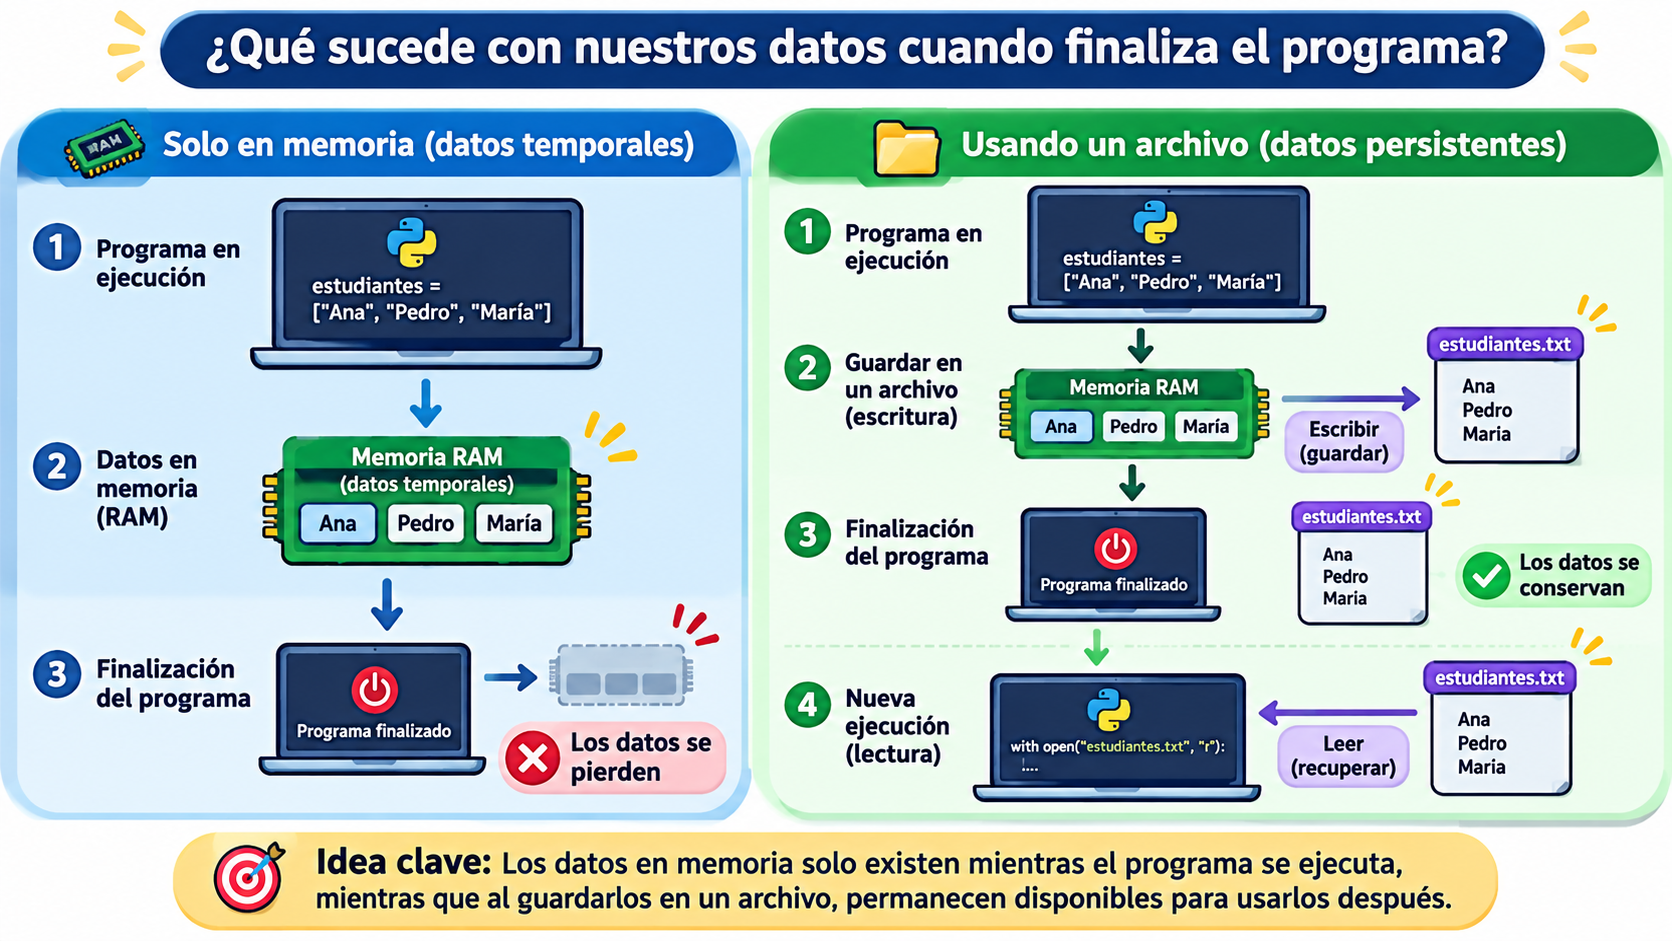
\includegraphics[width=\linewidth]{archivos_almacenamiento.png}
        \end{figure}
    \end{frame}


    \begin{frame}{Concepto}
        \begin{itemize}
            \item Un archivo es una unidad lógica de almacenamiento que permite conservar datos de forma persistente.
            \pause

            \item Los archivos permiten recuperar y procesar datos en diferentes ejecuciones de un programa.
            \pause

            \item Para identificar y describir un archivo, consideraremos tres elementos:
            \begin{itemize}
                \item \textbf{Nombre:} Permite identificar el archivo.
                \item \textbf{Extensión:} Suele indicar el formato
                de los datos almacenados.
                \item \textbf{Contenido:} Conjunto de datos
                almacenados en el archivo.
            \end{itemize}
        \end{itemize}
    \end{frame}

    \begin{frame}{Concepto}
        \renewcommand{\arraystretch}{1.5}
        \begin{center}
            \footnotesize
            \begin{tabular}{@{}p{3.8cm}p{6.5cm}@{}}
                \toprule
                \textbf{Archivo} & \textbf{Contenido} \\
                \midrule
                \texttt{estudiantes.txt} &
                Nombres de estudiantes \\
                \texttt{notas.csv} &
                Calificaciones organizadas en filas y columnas \\
                \texttt{configuracion.json} &
                Datos estructurados mediante claves y valores \\
                \texttt{imagen.png} &
                Información de una imagen \\
                \bottomrule
            \end{tabular}
        \end{center}
        \vspace{0.5em}
        \textbf{Nota:} La extensión no determina por sí sola el contenido real de un archivo.
    \end{frame}

    \begin{frame}{Utilidad de los archivos}
        \textcolor{red}{\textbf{Problema:}} Las variables de un programa se guardan en la memoria RAM, que es volátil. Por tanto,
        los datos se pierden al finalizar la ejecución del programa.
    \end{frame}

    \begin{frame}[fragile, t]{Utilidad de los archivos}
        \textcolor{red}{\textbf{Problema:}} Las variables de un programa se guardan en la memoria RAM, que es volátil. Por tanto,
        los datos se pierden al finalizar la ejecución del programa.
        
        
        \textcolor{green}{\textbf{Solución:}} Los archivos residen en almacenamiento secundario (disco, SSD), que no es volátil. Esto permite:
    \end{frame}

    \begin{frame}[fragile, t]{Utilidad de los archivos}
        \begin{itemize}
            \item Persistencia. Los datos se conservan entre ejecuciones y no dependen del ciclo de vida del programa. 
            \pause
            \item Procesamiento de volúmenes de datos. El programa obtiene sus datos de entrada desde un archivo y no mediante
            el ingreso manual con \mintinline{python}{input()}.
            \pause
            \item Interoperabilidad. Un formato estándar (.txt, .csv, .json, etc.) permite que distintos programas y sistemas lean 
            y escriban los mismos datos.
            \pause
            \item Almacenamiento de resultados. Los datos de salida de un programa se guardan para consultarlos o procesarlos después.
        \end{itemize}
    \end{frame}


    \begin{frame}[fragile, t]{Utilidad de los archivos}
        Sin archivos, los datos ingresan manualmente en cada ejecución:
        \begin{minted}[xleftmargin=-2cm, frame=leftline, fontsize=\small]{python}
            nota1 = float(input("Nota 1: "))
            nota2 = float(input("Nota 2: "))
            nota3 = float(input("Nota 3: "))
            # ¿Y si son 500 estudiantes?
        \end{minted}
        Con archivos, los datos se leen desde una fuente que ya existe:
        \begin{minted}[xleftmargin=-2cm, frame=leftline, fontsize=\small]{python}
            with open("notas.txt", "r") as archivo:
                for linea in archivo:
                    nota = float(linea.strip())
                    print(nota)
                    # procesa cada nota
        \end{minted}
    \end{frame}

    \begin{frame}[fragile, t]{Tipos de archivos}
        \renewcommand{\arraystretch}{1.35}
        \begin{center}
            \scriptsize
            \begin{tabular}{@{}p{2cm}p{4cm}p{4cm}@{}}
                \toprule
                & \textbf{Archivos de texto} & \textbf{Archivos binarios} \\
                \midrule
                Contenido &
                Bytes que representan caracteres según una codificación (UTF-8, ASCII) &
                Bytes que se interpretan según un formato específico \\
                Organización &
                Secuencia de caracteres organizada en líneas, separadas por \texttt{\textbackslash n} &
                Estructura definida por el formato (encabezados, bloques, compresión) \\
                Legibilidad &
                Se leen con cualquier editor de texto &
                Requieren un programa que conozca el formato \\
                Ejemplos &
                \texttt{.txt}, \texttt{.csv}, \texttt{.json}, \texttt{.py}, \texttt{.html} &
                \texttt{.png}, \texttt{.jpg}, \texttt{.mp3}, \texttt{.pdf}, \texttt{.xlsx}, \texttt{.exe} \\
                \bottomrule
            \end{tabular}
        \end{center}
    \end{frame}

    \begin{frame}[fragile, t]{Tipos de archivos}
        \begin{itemize}
            \item Texto plano (\texttt{.txt}): No tiene una estructura definida.
            \begin{minted}[xleftmargin=-2cm, frame=leftline, fontsize=\small]{bash}
            36.8
            37.1
            36.5
            \end{minted}
            \pause
            \item Valores separados por comas (\texttt{.csv}): Datos tabulares. Cada fila es un registro y cada columna es un campo separado por un delimitador (\texttt{,} o \texttt{;}).
            \begin{minted}[xleftmargin=-2cm, frame=leftline, fontsize=\small]{bash}
            nombre,edad,temperatura
            Ana,34,36.8
            Luis,52,37.1
            \end{minted}
            \pause
            \item Archivos JSON (\texttt{.json}): Datos jerárquicos estructurados mediante claves y valores.
            \begin{minted}[xleftmargin=-2cm, frame=leftline, fontsize=\small]{python}
            {"nombre": "Ana", "edad": 34, "mediciones": [36.8, 37.1]}
            \end{minted}
        \end{itemize}
    \end{frame}

    \begin{frame}[fragile, t]{Rutas de archivos}
        Una ruta de archivo es la dirección completa de un archivo en el sistema de archivos.
        \begin{itemize}
            \item Ruta absoluta: Parte desde la raíz del sistema.
            \begin{minted}[xleftmargin=-2cm, frame=leftline, fontsize=\small]{bash}
            C:/Users/user/cursos/datos/notas.txt      (Windows)
            /home/user/cursos/datos/notas.txt         (Linux / macOS)
            \end{minted}
            \pause
            \item Ruta relativa: Parte desde el directorio de trabajo actual.
            \begin{minted}[xleftmargin=-2cm, frame=leftline, fontsize=\small]{bash}
            notas.txt            → archivo en el directorio de trabajo
            datos/notas.txt      → archivo en la subcarpeta datos
            ../notas.txt         → archivo en la carpeta superior
            \end{minted}
        \end{itemize}
    \end{frame}

    \begin{frame}[fragile, t]{Apertura de archivos con \mintinline{python}{open()}}
        \begin{minted}[xleftmargin=-2cm, frame=leftline, fontsize=\small]{python}
            archivo = open(ruta, modo, encoding=codificacion)
        \end{minted}
        \begin{itemize}
            \item \texttt{ruta}: La ruta del archivo a abrir.
            \item \texttt{modo}: El modo de apertura del archivo (\texttt{r}, \texttt{w}, \texttt{a}).
            \item \texttt{encoding}: La codificación de caracteres (UTF-8, ASCII, etc.).
        \end{itemize}
        \renewcommand{\arraystretch}{1.4}
        \begin{center}
            \footnotesize
            \begin{tabular}{@{}p{1cm}p{1.5cm}p{3.5cm}p{3.5cm}@{}}
                \toprule
                \textbf{Modo} & \textbf{Operación} & \textbf{Si el archivo existe} & \textbf{Si no existe} \\
                \midrule
                \texttt{"r"} &
                Lectura &
                Lo abre desde el inicio &
                \texttt{FileNotFoundError} \\
                \texttt{"w"} &
                Escritura &
                Borra su contenido &
                Lo crea \\
                \texttt{"a"} &
                Agregar &
                Escribe al final, conservando el contenido &
                Lo crea \\
                \bottomrule
            \end{tabular}
        \end{center}
    \end{frame}

    \begin{frame}[fragile, t]{Cierre de archivos con \mintinline{python}{close()}}
        \begin{minted}[xleftmargin=-2cm, frame=leftline, fontsize=\small]{python}
            archivo = open("notas.txt", "r", encoding="utf-8")
            contenido = archivo.read()
            archivo.close()
        \end{minted}
        Cerrar un archivo:
        \begin{itemize}
            \item Libera el recurso: El sistema operativo limita la cantidad de archivos abiertos por un programa.
            \item Confirma la escritura: Al escribir, los datos se acumulan primero en un buffer en memoria. 
            El cierre transfiere ese contenido al disco. Si no se cierra, parte de los datos puede no quedar guardada.
        \end{itemize}
    \end{frame}

    \begin{frame}[fragile, t]{Apertura segura con \mintinline{python}{with}}
        \begin{minted}[xleftmargin=-2cm, frame=leftline, fontsize=\small]{python}
            with open("notas.txt", "r", encoding="utf-8") as archivo:
                contenido = archivo.read()
            # aquí el archivo ya está cerrado   
        \end{minted}
        \begin{itemize}
            \item El \mintinline{python}{with} abre el archivo y lo asigna a la variable indicada después del \mintinline{python}{as}.
            \item El bloque indentado define el alcance en que el archivo está abierto.
            \item Al salir del bloque, el archivo se cierra automáticamente.
        \end{itemize}
    \end{frame}

    \begin{frame}[fragile, t]{Métodos de lectura}
        \renewcommand{\arraystretch}{1.35}
        \begin{center}
            \scriptsize
            \begin{tabular}{@{}p{2.8cm}p{3.5cm}p{4cm}@{}}
                \toprule
                \textbf{Método} & \textbf{Retorna} & \textbf{Uso recomendado} \\
                \midrule
                \mintinline{python}{read()} &
                Un \mintinline{python}{str} con todo el contenido &
                Archivos pequeños que se procesan completos \\
                \mintinline{python}{readline()} &
                Un \mintinline{python}{str} con la línea siguiente, incluido \mintinline{python}{\textbackslash n} &
                Leer líneas específicas, como un encabezado \\
                \mintinline{python}{readlines()} &
                Una \mintinline{python}{list} de \mintinline{python}{str}, una por línea &
                Cuando se necesita acceder a las líneas por índice \\
                \mintinline{python}{for linea in archivo} &
                Un \mintinline{python}{str} por iteración &
                Recorrer archivos línea por línea (forma más usada) \\
                \bottomrule
            \end{tabular}
        \end{center}
    \end{frame}

    \begin{frame}[fragile, t]{\mintinline{python}{read()} y \mintinline{python}{readline()}}
        \begin{minted}[xleftmargin=-2cm, frame=leftline, fontsize=\small]{python}
            with open("temperaturas.txt", "r", encoding="utf-8") as archivo:
                contenido = archivo.read()
            print(repr(contenido))     # '36.8\n37.1\n36.5\n'
        \end{minted}

        \begin{minted}[xleftmargin=-2cm, frame=leftline, fontsize=\small]{python}
            with open("temperaturas.txt", "r", encoding="utf-8") as archivo:
                primera = archivo.readline()     # '36.8\n'
                segunda = archivo.readline()     # '37.1\n'
        \end{minted}

        Posición de lectura: el objeto archivo mantiene un cursor que avanza con cada lectura.

        \begin{itemize}
            \item Cada \mintinline{python}{readline()} continúa donde terminó la lectura anterior.
            \item Después de \mintinline{python}{read()}, el cursor queda al final: una segunda llamada retorna ''.
            \item \mintinline{python}{readline()} retorna \mintinline{python}{''} cuando se alcanza el fin del archivo.
        \end{itemize}
    \end{frame}

    \begin{frame}[fragile, t]{\mintinline{python}{readlines()} e iteración con \mintinline{python}{for}}
        \begin{minted}[xleftmargin=-2cm, frame=leftline, fontsize=\small]{python}
            with open("temperaturas.txt", "r", encoding="utf-8") as archivo:
                lineas = archivo.readlines()
            print(lineas)     # ['36.8\n', '37.1\n', '36.5\n']
        \end{minted}

        \begin{minted}[xleftmargin=-2cm, frame=leftline, fontsize=\small]{python}
            with open("temperaturas.txt", "r", encoding="utf-8") as archivo:
                for linea in archivo:
                    print(linea)    
        \end{minted}

        \begin{itemize}
            \item \mintinline{python}{readlines()} carga todas las líneas en memoria a la vez.
            \item La iteración con \mintinline{python}{for} una línea a la vez, por lo que es más eficiente con archivos grandes.
        \end{itemize}
    \end{frame}
\end{document}